%%%%%%%%%%%%%%%%%%%%%%%%%%%%%%%%%%%%%%%%%%%%%%%%%%%%%%%%
%                IAML 2020 Assignment 2                %
%                                                      %
%                                                      %
% Authors: Hiroshi Shimodaira and JinHong Lu           %
% Based on: Assignment 1 by Oisin Mac Aodha, and       %
%          Octave Mariotti                             %
% Using template from: Michael P. J. Camilleri and     %
% Traiko Dinev.                                        %
%                                                      %
% Based on the Cleese Assignment Template for Students %
% from http://www.LaTeXTemplates.com.                  %
%                                                      %
% Original Author: Vel (vel@LaTeXTemplates.com)        %
%                                                      %
% License:                                             %
% CC BY-NC-SA 3.0                                      %
% (http://creativecommons.org/licenses/by-nc-sa/3.0/)  %
%                                                      %
%%%%%%%%%%%%%%%%%%%%%%%%%%%%%%%%%%%%%%%%%%%%%%%%%%%%%%%%

%--------------------------------------------------------
%   IMPORTANT: Do not touch anything in this part
\documentclass[12pt]{article}
\input{style.tex}



% Options for Formatting Output

\global\setbool{clearon}{true} %
\global\setbool{authoron}{true} %
\ifbool{authoron}{\rhead{\small{\assignmentAuthorName}}\cfoot{\small{\assignmentAuthorName}}}{\rhead{}}



\newcommand{\assignmentQuestionName}{Question}
\newcommand{\assignmentTitle}{Assignment\ \#2}

\newcommand{\assignmentClass}{IAML -- INFR10069 (LEVEL 10)}

\newcommand{\assignmentWarning}{NO LATE SUBMISSIONS} % 
\newcommand{\assignmentDueDate}{Monday,\ November\ 23,\ 2020 @ 16:00}
%--------------------------------------------------------



%%%%%%%%%%%%%%%%%%%%%%%%%%%%%%%%%%%%%%%%%%%%%%%%%%%%%%%
%
% NOTE: YOU NEED TO ENTER YOUR STUDENT ID BELOW.
%
%%%%%%%%%%%%%%%%%%%%%%%%%%%%%%%%%%%%%%%%%%%%%%%%%%%%%%%% 
% --------------------------------------------------------
% IMPORTANT: Specify your Student ID below. You will need to uncomment the line, else compilation will fail. Make sure to specify your student ID correctly, otherwise we may not be able to identify your work and you will be marked as missing.
\newcommand{\assignmentAuthorName}{s1864480}
%--------------------------------------------------------



\begin{document}


%%%%%%%%%%%%%%%%%%%%%%%%%%%%%%%%%%%%%%%%%%%%%%%%%%%%%%%%%%%%%%%%%%%%%%%%%%%%%%
%============================================================================%
%%%%%%%%%%%%%%%%%%%%%%%%%%%%%%%%%%%%%%%%%%%%%%%%%%%%%%%%%%%%%%%%%%%%%%%%%%%%%%
\clearpage
%
% Question 1
%

\begin{question}{(30 total points) Image data analysis with PCA}

  
  \questiontext{In this question we employ PCA to analyse image data}
  

  
  \medskip

   %==============================
   % Q1.1
  \begin{subquestion}{(3 points)
      Once you have applied the normalisation from Step 1 to Step 4 above,
      report the values of the first 4 elements for the first training
      sample in \texttt{Xtrn\_nm},
      i.e. \texttt{Xtrn\_nm[0,:]} and the last training sample,
      i.e. \texttt{Xtrn\_nm[-1,:]}.
    } \label{Q1.1}
    

      \begin{answerbox}{10em}
         The first 4 elements of the first and the last training sample are:
         $$[-0.    , -0.    , -0.0001, -0.0004]$$
      \end{answerbox}
  


   \end{subquestion}
   %
   % ==============================
   % 
   % Q1.2
   \begin{subquestion}{(4 points)
      Using {\tt Xtrn} and Euclidean distance
      measure, for each class,
      find the two closest samples and two furthest
      samples of that class to the mean vector of the class.
    }  \label{Q1.2}




  \begin{answerbox}{52em}
    \begin{center}
        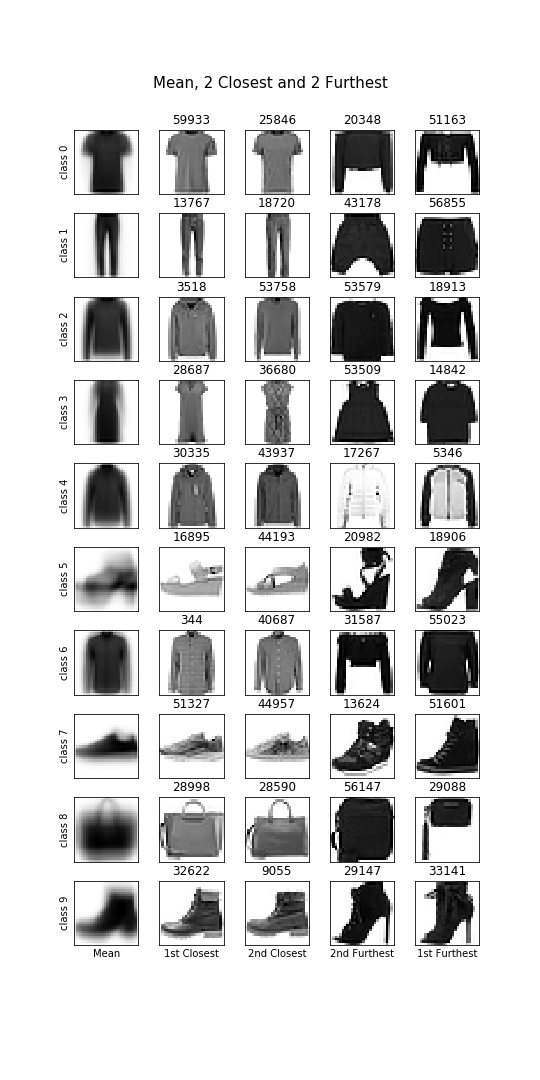
\includegraphics[width=0.65\textwidth]{results/1_2.png}
    \end{center}
  \end{answerbox}



   \end{subquestion}

   % 
   % Q1.3
   \begin{subquestion}{(3 points)
       Apply Principal Component Analysis (PCA) to the data of {\tt
         Xtrn\_nm} using
       \href{https://scikit-learn.org/0.19/modules/generated/sklearn.decomposition.PCA.html}{sklearn.decomposition.PCA},
       and report the variances of projected data for the first five principal
       components in a table. Note that you should use {\tt Xtrn\_nm} instead of {\tt Xtrn}.} 
    \label{Q1.pca.variance}
     


    \begin{answerbox}{15em}
        \centering
        \begin{tabular}{|c|l|}
            \hline
            \multicolumn{1}{|l|}{\textbf{Principal Component (PC)}} & \textbf{Variance} \\ \hline
            PC1                                            & 19.8098  \\ \hline
            PC2                                            & 12.1122  \\ \hline
            PC3                                            & 4.1062   \\ \hline
            PC4                                            & 3.3818   \\ \hline
            PC5                                            & 2.624    \\ \hline
        \end{tabular}
    \end{answerbox}
    


   \end{subquestion}

   %==============================
   % Q1.4
   \begin{subquestion}{(3 points)
       Plot a graph of the cumulative explained variance ratio as a
       function of the number of principal components, $K$, where $1
       \le K \le 784$.
       Discuss the result briefly.
       } \label{Q1.plot.pca.variance}
   

      \begin{answerbox}{30em}
        \begin{center}
            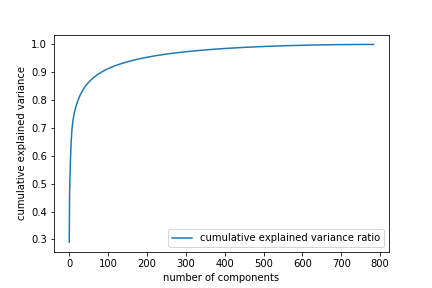
\includegraphics[width=0.75\textwidth]{results/1_4.png}
        \end{center}
        This curve shows how much of the total, 784-dimensional variance is contained within the first $N$ components. Here we can see that in the dataset the first $100$ components contain approximately $90\%$ of the variance, while we need around $500$ components to describe close to $100\%$ of the variance. This allows us to work with and explore the dataset more easily, as we can project our $784$ to much smaller dimensions, for eg. $100$. 
      \end{answerbox}
  


   \end{subquestion}

   %==============================
   % Q1.5
   \begin{subquestion}{(4 points)
      Display the images of the first 10 principal components in
      a 2-by-5 grid, putting the image of 1st principal component on
      the top left corner, followed by the one of 2nd component to the right.
      Discuss your findings briefly.
     } \label{Q1.disp.pca}
   

      \begin{answerbox}{35em}
         \begin{center}
            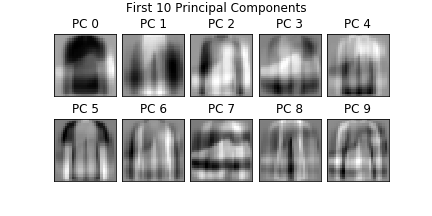
\includegraphics[width=0.7\textwidth]{results/1_5.png}
        \end{center}
      \end{answerbox}
  


   \end{subquestion}

   %==============================
   % Q1.6
   \begin{subquestion}{(5 points)
       Using \texttt{Xtrn\_nm}, 
       for each class and for each number of principal components $K =
       5, 20, 50, 200$, apply dimensionality reduction with PCA to the
       first sample in the class, reconstruct the sample from the
       dimensionality-reduced sample, and 
       report the Root Mean Square Error (RMSE) between the
       original sample in {\tt Xtrn\_nm} and reconstructed one.
     } \label{Q1.6}

     

      \begin{answerbox}{25em}
         \centering
        \begin{tabular}{|c|l|l|l|l|l|l|l|l|}
            \hline
            \textbf{Class} & \textbf{K} & \textbf{RSME} & \textbf{K} & \textbf{RSME} & \textbf{K} & \textbf{RSME} & \textbf{K} & \textbf{RSME}   \\ \hline
            0     & 5 & 0.2561 & 20 & 0.1501 & 50 & 0.127 & 200 & 0.0619 \\ \hline
            1     & 5 & 0.198 & 20 & 0.1404 & 50 & 0.0952 & 200 & 0.0361 \\ \hline
            2     & 5 & 0.1987 & 20 & 0.1455 & 50 & 0.1224 & 200 & 0.0798 \\ \hline
            3     & 5 & 0.1457 & 20 & 0.1075 & 50 & 0.0838 & 200 & 0.0561 \\ \hline
            4     & 5 & 0.1182 & 20 & 0.1026 & 50 & 0.087 & 200 & 0.0466 \\ \hline
            5     & 5 & 0.1811 & 20 & 0.1586 & 50 & 0.1431 & 200 & 0.0898 \\ \hline
            6     & 5 & 0.1295 & 20 & 0.0963 & 50 & 0.0725 & 200 & 0.0446 \\ \hline
            7     & 5 & 0.1656 & 20 & 0.1272 & 50 & 0.1059 & 200 & 0.0614 \\ \hline
            8     & 5 & 0.2234 & 20 & 0.1449 & 50 & 0.1233 & 200 & 0.093 \\ \hline
            9     & 5 & 0.1835 & 20 & 0.1513 & 50 & 0.1218 & 200 & 0.0716 \\ \hline
        \end{tabular}
      \end{answerbox}
  


   \end{subquestion}
   
   %==============================
   % Q1.7
   \begin{subquestion}{(4 points)
       Display the image for each of the reconstructed samples in
       a 10-by-4 grid, where each row corresponds to a class and
       each row column corresponds to a value of $K=5, \; 20, \; 50, \; 200$.
     } \label{Q1.7}


   

      \begin{answerbox}{52em}
         \begin{center}
             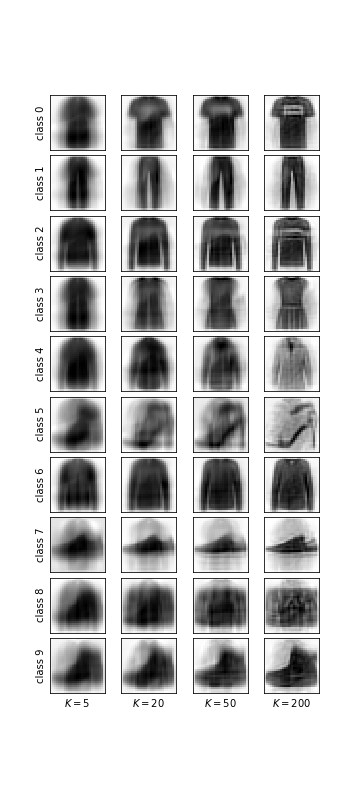
\includegraphics[scale=0.75]{results/1_7.png}
         \end{center}
      \end{answerbox}
  


   \end{subquestion}
   %==============================
   %
   %==============================
   % Q1.8
   \begin{subquestion}{(4 points)
       Plot all the training samples (\texttt{Xtrn\_nm}) on the
       two-dimensional PCA plane you obtained in \refQ{Q1.pca.variance}, where each sample is
       represented as a small point with a colour specific to the class of
       the sample.  Use the 'coolwarm' colormap for plotting.
     } \label{Q1.8}


   

      \begin{answerbox}{40em}
         \begin{center}
             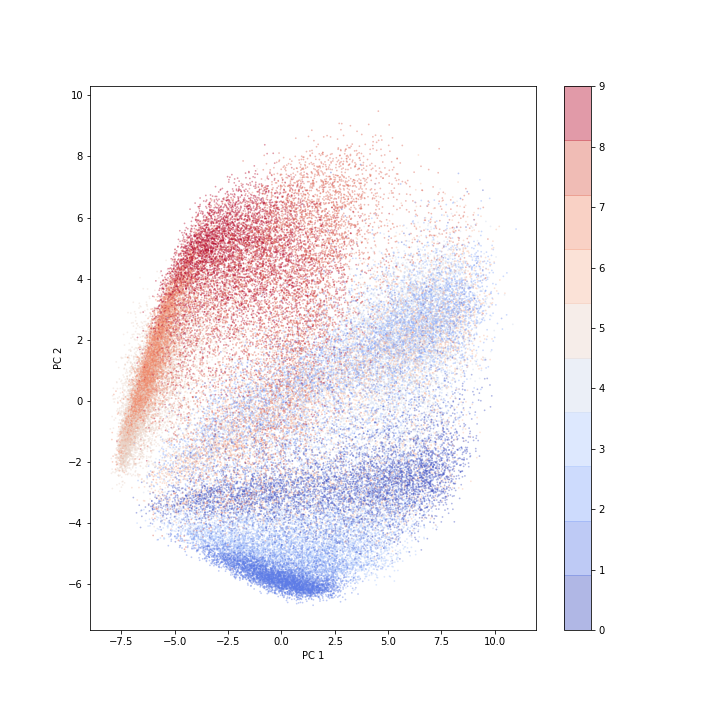
\includegraphics[width=0.9\textwidth]{results/1_8.png}
         \end{center}
      \end{answerbox}
  


   \end{subquestion}
   %
   %==============================
   

\end{question}
%%%%%%%%%%%%%%%%%%%%%%%%%%%%%%%%%%%%%%%%%%%%%%%%%%%%%%%%%%%%%%%%%%%%%%%%%%%%%%
%============================================================================%
%%%%%%%%%%%%%%%%%%%%%%%%%%%%%%%%%%%%%%%%%%%%%%%%%%%%%%%%%%%%%%%%%%%%%%%%%%%%%%
\clearpage
%
% Question 2
%
\begin{question}{(25 total points) Logistic regression and SVM}

  \questiontext{In this question we will explore 
    classification of image data with logistic regression and support
    vector machines (SVM) and visualisation 
    of decision regions.
  }
  


  \medskip
   %==============================
   % Q2.1
   \begin{subquestion}{(3 points)
       Carry out a classification experiment with
       \href{https://scikit-learn.org/0.19/modules/generated/sklearn.linear\_model.LogisticRegression.html}{multinomial logistic regression},
       and report the classification accuracy and confusion matrix (in
       numbers rather than in graphical representation such as heatmap)
       for the test set.
     } \label{Q2.1}


   

      \begin{answerbox}{30em}
         Your Answer Here
      \end{answerbox}
  


   \end{subquestion}
   %
   % ==============================
   %
   %==============================
   % Q2.2
   \begin{subquestion}{(3 points)
       Carry out a classification experiment with
       \href{https://scikit-learn.org/0.19/modules/generated/sklearn.svm.SVC.html}{SVM classifiers}, and report the
       mean accuracy and confusion matrix (in numbers) for the test
       set.
     } \label{Q2.2}


   

      \begin{answerbox}{30em}
         Your Answer Here
      \end{answerbox}
  


   \end{subquestion}
   %
   % ==============================
   %
   %==============================
   % Q2.3
   \begin{subquestion}{(6 points)
       We now want to visualise the decision regions for the logistic
       regression classifier we trained in \refQ{Q2.1}.
     } \label{Q2.3}


   

      \begin{answerbox}{35em}
         Your Answer Here
      \end{answerbox}
  


   \end{subquestion}
   %
   % ==============================
   %
   %==============================
   % Q2.4
   \begin{subquestion}{(4 points)
       Using the same method as the one above, plot the decision regions for
       the SVM classifier you trained in \refQ{Q2.2}.
       Comparing the result with that you obtained in \refQ{Q2.3}, discuss your
       findings briefly.
     } \label{Q2.4}
   

      \begin{answerbox}{35em}
         Your Answer Here
      \end{answerbox}
  


   \end{subquestion}
   %
   % ==============================
   %

   %==============================
   % Q2.5
   \begin{subquestion}{(6 points)
       We used default parameters for the SVM in \refQ{Q2.2}.
       We now want to tune the parameters by using cross-validation.
       To reduce the time for experiments, you pick up the first 1000
       training samples from each class to create \texttt{Xsmall}, so that \texttt{Xsmall}
       contains 10,000 samples in total. Accordingly, you create
       labels, \texttt{Ysmall}.
     } \label{Q2.5}


   

      \begin{answerbox}{30em}
         Your Answer Here
      \end{answerbox}
  


   \end{subquestion}
   %
   % ==============================
   %
   %==============================
   % Q2.6
   \begin{subquestion}{(3 points)
       Train the SVM classifier on the whole training set by using the
       optimal value of $C$ you found in \refQ{Q2.5}. 
     } \label{Q2.6}


       

      \begin{answerbox}{10em}
         Your Answer Here
      \end{answerbox}
  


   \end{subquestion}
   %
   % ==============================
   %
%
%

\end{question}
%%%%%%%%%%%%%%%%%%%%%%%%%%%%%%%%%%%%%%%%%%%%%%%%%%%%%%%%%%%%%%%%%%%%%%%%%%%%%%
%============================================================================%
%%%%%%%%%%%%%%%%%%%%%%%%%%%%%%%%%%%%%%%%%%%%%%%%%%%%%%%%%%%%%%%%%%%%%%%%%%%%%%
\clearpage
%
% Question 3
%

\begin{question}{(20 total points) Clustering and Gaussian Mixture Models}  


  \questiontext{In this question we will explore K-means clustering,
    hierarchical clustering, and GMMs.
  }
  


  \medskip
   %==============================
   % Q3.1
   \begin{subquestion}{(3 points)
       Apply k-means clustering on {\tt Xtrn} for $k = 22$, where we use
       \href{https://scikit-learn.org/0.19/modules/generated/sklearn.cluster.KMeans.html}{sklearn.cluster.KMeans}
       with the parameters {\tt n\_clusters=22} and {\tt random\_state=1}.
       Report the sum of squared distances of samples to their closest
       cluster centre, and the number of samples for each cluster.
     } \label{Q3.1}
   

      \begin{answerbox}{35em}
         Your Answer Here
      \end{answerbox}
  


   \end{subquestion}
   %
   % ==============================
   %
   %==============================
   % Q3.2
   \begin{subquestion}{(3 points)
       Using the training set only,
       calculate the mean vector for each language, and plot the mean
       vectors of all the 22 languages on a 2D-PCA plane, where you
       apply PCA on the set of 22 mean vectors without applying
       standardisation.  
       On the same figure, plot the cluster centres obtained in \refQ{Q3.1}.
     } \label{Q3.2}

   

      \begin{answerbox}{35em}
         Your Answer Here
      \end{answerbox}
  


   \end{subquestion}
   %
   % ==============================
   %
   %==============================
   % Q3.3
   \begin{subquestion}{(3 points)
       We now apply hierarchical clustering on the training data set
       to see if there are any structures in the spoken languages.
     } \label{Q3.3}


     

      \begin{answerbox}{35em}
         Your Answer Here
      \end{answerbox}
  


   \end{subquestion}
   %
   % ==============================
   %
   %==============================
   % Q3.4
   \begin{subquestion}{(5 points)
       We here extend the hierarchical clustering done in \refQ{Q3.3} by
       using multiple samples from each language.
     } \label{Q3.4}


   

      \begin{answerbox}{50em}
         Your Answer Here
      \end{answerbox}
  


   \end{subquestion}
   %
   % ==============================
   %
   %==============================
   % Q3.5
   \begin{subquestion}{(6 points)
       We now consider Gaussian mixture model (GMM), whose
       probability distribution function (pdf) is given as
       a linear combination of Gaussian or normal distributions, i.e.,
     } \label{Q3.5}




      \begin{answerbox}{30em}
         Your Answer Here
      \end{answerbox}
  


   \end{subquestion}
   %
   %==============================

   % ==============================
   
\end{question}
\end{document}
